\chapter{Paper} \label{c:Paper}
In this chapter we will examine the topic of the paper \textit{Stable Neo-Hookean Flesh Simulation} \cite{Smith:2018:SNF:3191713.3180491}. In the interest of understanding the thought process of the authors I will include some of their calculations a bit more detailed. In addition examples and visualisations should help for a better perception. 

\section{Deformation Gradient}

\begin{table}[!htbp]
\centering
    \begin{tabular}{ | l | l |}
    \hline
    \textbf{Symbol} & \textbf{Definition} \\ \hline
    $\mathrm{F=RS}$ & Polar decomposition \\ \hline
    $J=\operatorname{det}(\mathrm{F})$ & Relative volume change \\ \hline
    $\mathrm{C}=\mathrm{F}^{T} \mathrm{F}$ & Right Cauchy-Green  \\ \hline	
    $I_{C}=\operatorname{tr}(\mathrm{C})$ & First right Cauchy-Green invariant \\ \hline
    \end{tabular}
    \caption{Quantities Derived from the Deformation Gradient \textbf{F} taken from \cite{Smith:2018:SNF:3191713.3180491}}
\label{table:1}
\end{table}

\todoredefined[inline]{
TODO: Add in Background? Explain more each entity
}


\section{Energy Formulation}

\subsection{Stability}
The core goal of the paper was to model deformations for virtual characters that have human-like features. They concentrated on the deformation energy. In order to achieve a convincing result as a first step we need to specify some requirements. For our needs in this case the stability of the energy is important. More precisely we need a hyperelastic energy that is stable in the following four important ways:

\textbf{1. Inversion Stability:} Given some arbitrary object it is possible that while deforming the object we can arrive at a zero volume state or even an entire inversion. Take for example the tetrahedron shown in figure \ref{fig:inversion_1}. In figure \ref{fig:inversion_2} we see a deformed state of this tetrahedron where the volume is scaled down to zero and we are left with a simple triangle. In figure \ref{fig:inversion_3} image we have an inversion of the object. The needed deformation energy has to be able to deal with both cases. That means that the energy has to be singularity-free and does not need any filters or threshold (\cite{Smith:2018:SNF:3191713.3180491}, 12:3).

\todoredefined[inline]{
TODO: Explain what last sentence means. Reference correct like this?
}

\begin{figure}[!ht]
\centering
\begin{subfigure}{.3\textwidth}
  \centering
  % include first image
  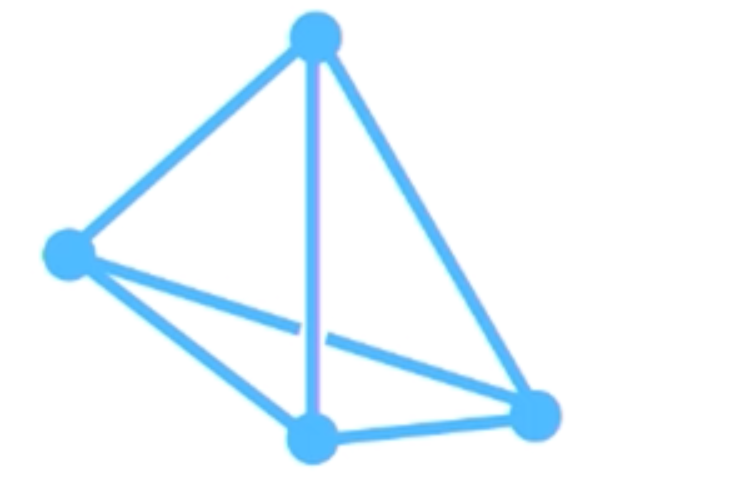
\includegraphics[width=.8\linewidth]{resources/inversion_1}  
  \caption{Rest state}
  \label{fig:inversion_1}
\end{subfigure}
\begin{subfigure}{.3\textwidth}
  \centering
  % include first image
  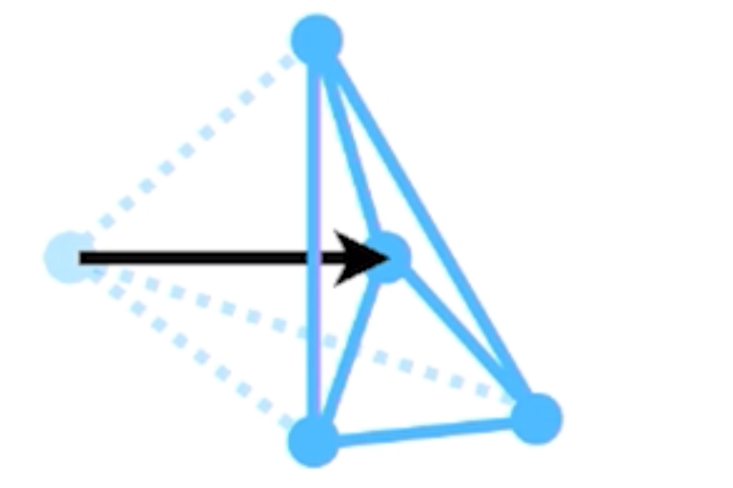
\includegraphics[width=.8\linewidth]{resources/inversion_2}  
  \caption{Zero-volume state}
  \label{fig:inversion_2}
\end{subfigure}
\begin{subfigure}{.3\textwidth}
  \centering
  % include second image
  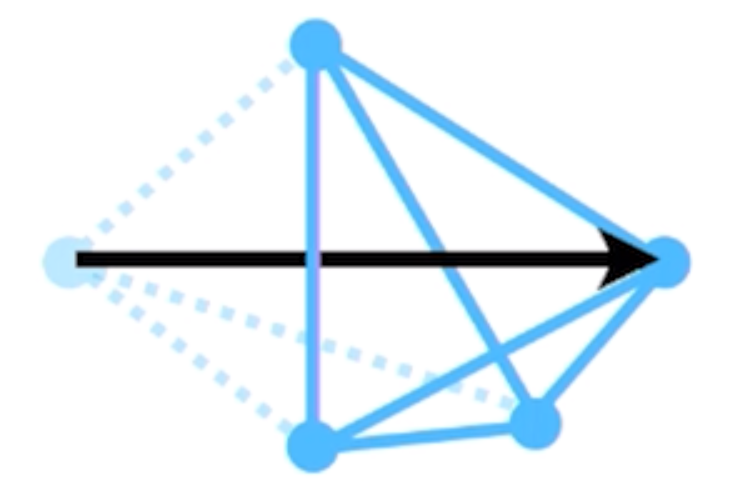
\includegraphics[width=.8\linewidth]{resources/inversion_3}  
  \caption{Inversed state}
  \label{fig:inversion_3}
\end{subfigure}
\caption{Inversion of a tetrahedron {\cite{STREAM2018}}}
\label{fig:inversion}
\end{figure}


\textbf{2. Reflection stability:} A reflection is rotation around the coordinate origin.
For the deformation energy we need it to be well behaved regardless of the reflection convention used in the singular value decomposition.

\textbf{3. Rest stability:} When deforming an object in a certain way we apply one or multiple forces over that object. With rest stability we want that if the sum of forces is equal to zero the object must be back in its rest state.

\textbf{4. Meta-stability under degeneracy:} We can crush an object into an arbitrary shape like a plane, line or point. That process is illustrated for a cube in figure \ref{fig:meta_stability}. The cube should now be able to recover to its actual shape after the deformation.

\begin{figure}[!htbp]
	\centering
	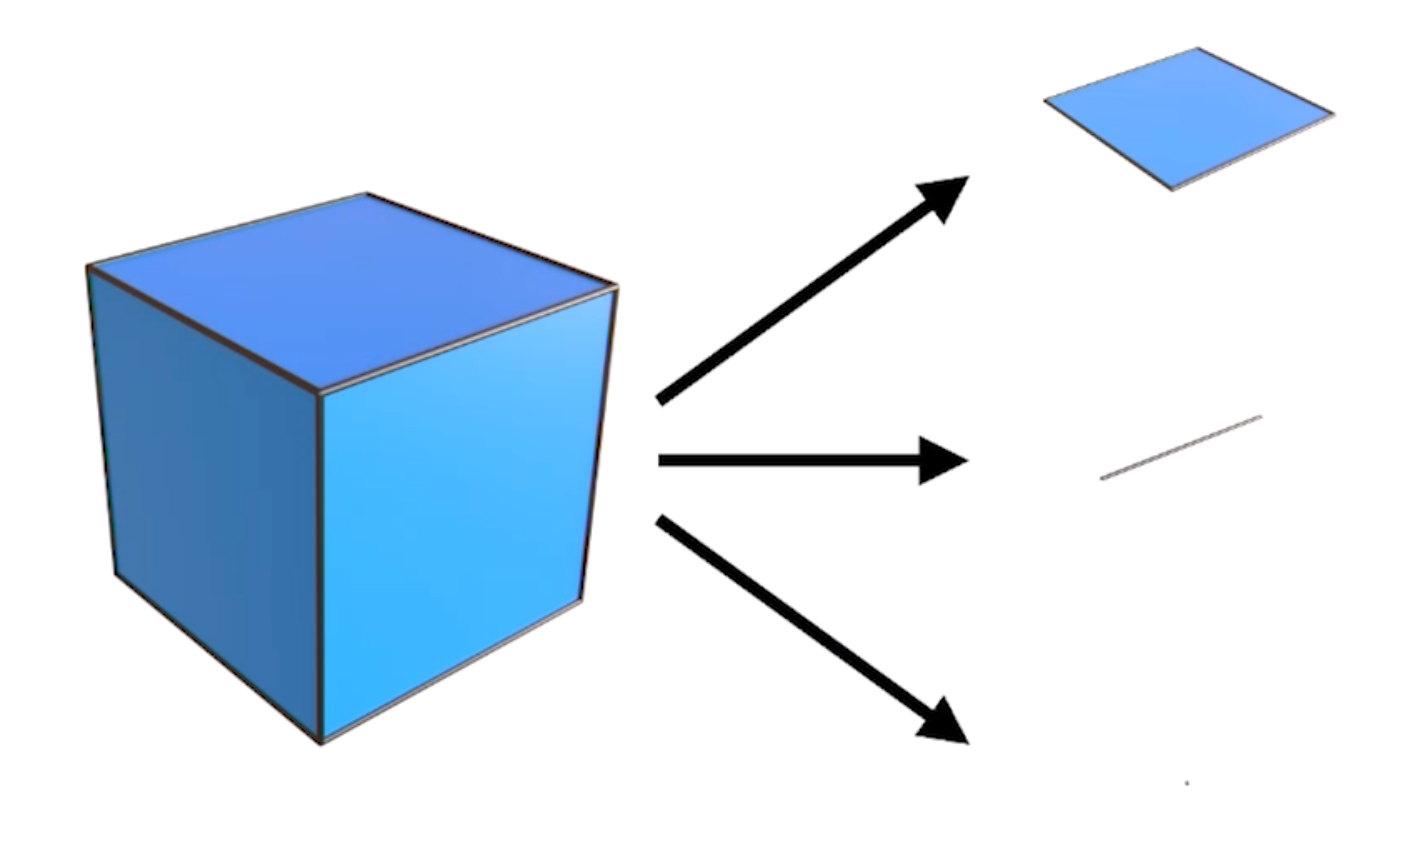
\includegraphics[width=0.5\textwidth]{resources/meta_stability}
	\caption{Illustration of meta stability {\cite{STREAM2018}}}
	\label{fig:meta_stability}
\end{figure}

Based on these four requirements we will in the following determine if a deformation energy is suited for our needs.

\todoredefined[inline]{
TODO: Finish reflection stability. Maybe add own images? Some more sources?
}

\subsection{Existing Neo-Hookean Energies}

In previous literature a few energies were proposed.

\begin{table}[!htbp]
\centering
    \begin{tabular}{ | l | l |}
    \hline
    \textbf{Energy} & \textbf{Author(s)} \\ \hline
    $\Psi_{Neo}=\frac{\mu}{2}\left(I_{C}-3\right)-\mu \log J+\frac{\lambda}{2}(\log J)^{2}$ & e.g. Bonet and Wood 2008 \\ \hline
    $\Psi_{\mathrm{A}}=\frac{\mu}{2}\left(I_{C}-3\right)-\mu \log J+\frac{\lambda}{2}(J-1)^{2}$ & Odgen 1997 \\ \hline
    $\Psi_{\mathrm{B}}=\frac{\mu}{2}\left(J^{-2 / 3} I_{C}-3\right)+\frac{\lambda}{2}(J-1)^{2}$ & Bower 2009 \\ \hline
    $\Psi_{\mathrm{C}}=\frac{\mu}{2}\left(J^{-2 / 3} I_{C}-3\right)+\frac{\lambda}{2}(J-1)^{2}$ & Wang and Yang 2016 \\ \hline
    \end{tabular}
    \caption{Summary of proposed energies taken from \cite{Smith:2018:SNF:3191713.3180491}}
\label{table:1}
\end{table}

Each energy formulation can be split up into a 1D length term and a 3D volume term.

\begin{table}[!htbp]
\centering
    \begin{tabular}{ | l | l | l |}
    \hline
    \textbf{Energy} & \textbf{1D length term} & \textbf{3D volume term} \\ \hline
    $\Psi_{Neo}$ & $\frac{\mu}{2}\left(I_{C}-3\right)$ & $-\mu \log J+\frac{\lambda}{2}(\log J)^{2}$ \\ \hline
    $\Psi_{\mathrm{A}}$ & $\frac{\mu}{2}\left(I_{C}-3\right)$ & $-\mu \log J+\frac{\lambda}{2}(J-1)^{2}$ \\ \hline
    $\Psi_{\mathrm{B}}$ & $\frac{\mu}{2}\left(J^{-2 / 3} I_{C}-3\right)$ & $\frac{\lambda}{2}(J-1)^{2}$ \\ \hline
    $\Psi_{\mathrm{C}}$ & $\frac{\mu}{2}\left(J^{-2 / 3} I_{C}-3\right)$ & $\frac{\lambda}{2}(J-1)^{2}$ \\ \hline
    \end{tabular}
    \caption{Energies split up into its 1D length and 3D volume term}
\label{table:1}
\end{table}

\textbf{1D Length Term:} This term penalizes length changes. Mooney (\cite{mooney1940theory}) originally proposed the 1D length term 
\[
\Psi_{M}=\frac{\mu}{2}\left(I_{C}-3\right)
\]
that is used in $\Psi_{Neo}$ and $\Psi_{A}$. If we expand the energy with the singular values of the deformation gradient \textbf{F} we get the following term:
\[
\Psi_{M}=\frac{\mu}{2}\left(\sigma_{0}^2 + \sigma_{1}^2 + \sigma_{2}^2 - 3\right)
\]
The energy as it is formulated reaches its minimum at a zero volume change, meaning $I_{C}=0$ which results in $\Psi_{M}=-3$. Mooney added the hard constraint that $J=1$ so that the energy is minimized at the volume preserving configuration. Note that the energy is singularity free and well defined under inversion.

The second term 
\[
\Psi_{R} = \frac{\mu}{2}\left(J^{-2 / 3} I_{C}-3\right)
\]
is used in $\Psi_{B}$ and $\Psi_{C}$ was introduced by Rivlin in 1948. Using the singular values of F we get the following term:
\[
\Psi_{R} = \frac{\mu}{2}\left(\frac{\sigma_{0}^2 + \sigma_{1}^2 + \sigma_{2}^2}{(\sigma_{0}  \sigma_{1}  \sigma_{2})^\frac{2}{3}}
 - 3\right)
\]
Unfortunately this term is not singularity free. If either $\sigma_{0}$, $\sigma_{1}$ or $\sigma_{2}$ is equal to zero the result is not defined anymore.


\textbf{3D Volume Term:} Here we are dealing with a volume-preserving penalty term. The volume term of $\Psi_{Neo}$, meaning
\[
\Psi_{Neo, volume} = -\mu \log J+\frac{\lambda}{2}(\log J)^{2}
\]
results in some numerical problems since the logarithmic function is not defined for $J<0$ and grows unbounded for $J \rightarrow 0$. In conclusion $\Psi_{Neo, volume}$ is not singularity free. 
The same applies for the 3D volume term of $\Psi_{A}$
\[
\Psi_{A, volume} = -\mu \log J+\frac{\lambda}{2}(J-1)^{2}.
\]
The term of $\Psi_{A}$ and $\Psi_{B}$
\[
\Psi_{M} = \frac{\lambda}{2}(J-1)^{2}
\]
does not have these noted difficulties. It is bounded, well defined and invertible. After these observations we combine the robust length with the robust volume term
\[
\Psi_{D} = \frac{\mu}{2}\left(I_{C}-3\right) +\frac{\lambda}{2}(J-1)^{2}
\]
which is singularity free and well defined under inversion.

\todoredefined[inline]{
TODO: Bonet and Wood 2008 or 1997? Table looks ugly, improve and add resources. minimum at IC=0 or J=0? Overall okay?
}

\subsection{Rest Stabilization}
Although $\Psi_{D}$ meets almost all of our requirements it is not rest stable. This can be shown with the Piola-Kirchhoff (PK1) stress tensor:
\[
P_{D}(I) = \frac{\partial \Psi_{D}}{\partial F} (I) = \frac{\partial \Psi_{D}}{\partial F} \left[ \frac{\mu}{2}\left(I_{C}-3\right) +\frac{\lambda}{2}(J-1)^{2} \right]
\]
\[
= \frac{\partial \Psi_{D}}{\partial F}  \frac{\mu}{2}\left(\operatorname{tr}(\mathrm{I}^{T} \mathrm{I})-3\right) +\frac{\partial \Psi_{D}}{\partial F} \frac{\lambda}{2}(\operatorname{tr}(\mathrm{I})-1)^{2}
\]
\[
= \mu I + \lambda (\operatorname{det}(I)-1)  \frac{\partial}{\partial F} \operatorname{det}(I) = \mu I \neq 0
\]

If the energy had rest stability $P_{D}(I)$ would resolve to zero. Unfortunately this is not the case here. In order to solve that problem the authors modified $(J-1)^{2}$ to $(J-\alpha)^{2}$:
\[
\Psi_{E} = \frac{\mu}{2}\left(I_{C}-3\right) +\frac{\lambda}{2}(J-\alpha)^{2}
\]
therefore resulting to:
\[
P_{E}(F) = \frac{\partial \Psi_{D}}{\partial F} \left[ \frac{\mu}{2}\left(I_{C}-3\right) +\frac{\lambda}{2}(J-\alpha)^{2} \right]
\]
\begin{equation}\label{eq:pk1_unstable}
= \mu F + \lambda (\operatorname{det}(F)-\alpha)  \frac{\partial}{\partial F} \operatorname{det}(F)
\end{equation}

Solving for an alpha that satisfies $P_{E}(I)=0$ gives us $\alpha=1+\frac{\mu}{\lambda}$. Now $\Psi_{E}$ has to be changed accordingly:
\[
\Psi_{E} = \frac{\mu}{2}\left(I_{C}-3\right) +\frac{\lambda}{2}(J-1-\frac{\mu}{\lambda})^{2}
\]
\[
= \frac{\mu}{2}\left(I_{C}-3\right) - \mu\left(J-1\right) + \frac{\lambda}{2}(J-1)^{2} + \left(\frac{\mu}{\lambda}\right)^{2}
\]
Since constant disappear under differentiation this expression is functionally equivalent to 
\[
\Psi_{E} = \frac{\mu}{2}\left(I_{C}-3\right) - \mu\left(J-1\right) + \frac{\lambda}{2}(J-1)^{2}.
\]
Now one can notice that $\Psi_{E}$ looks very similar to $\Psi_{Neo}$. The difference is that we replaced $log(J)$ with $(J-1)$ in $\Psi_{E}$. Remember that $(J-1)$ is the first term in the taylor approximation of $log(J)$ at $J=1$:
\[
\sum_{n=0}^{\infty} = \frac{f^{(n)}(1)}{n!} (J-1)^{n} =
\]
\[
= \boldsymbol{(J-1)} - \frac{1}{2} (J-1)^{2} + \frac{1}{3} (J-1)^{3} -\frac{1}{4} (J-1)^{4} + ...
\]

\todoredefined[inline]{
TODO: Add "Zwischenschritte"? Include all calculations? Do we need a bit of a better conclusion of what we did (taylor, neo, sing. free, rest stable)?
}

\subsection{Meta-Stability under Degeneracy}
The final energy is
\begin{equation}\label{eq:stable_energy}
\Psi_{new} = \frac{\mu}{2}\left(I_{C}-3\right) + \frac{\lambda}{2}(J-\alpha)^{2} - \frac{\mu}{2} \operatorname{log}\left(I_{C}+1\right).
\end{equation}
With that adjustment the rest stability term shifts to $\alpha=1+\frac{\mu}{\lambda}-\left(\frac{\mu}{4}\right)\lambda$.

\todoredefined[inline]{
TODO: How much needs to be explained here?
}

\subsection{Lamé Reparametrization}
\todoredefined[inline]{
TODO: How much needs to be explained here?
}


\section{Energy Analysis}
In this chapter it is shown that one can perform a complete eigenanalysis on equation \ref{eq:stable_energy}.

\subsection{First Piola-Kirchhoff Stress (PK1)}
We start with PK1 for equation \ref{eq:stable_energy}:
\[
P(F) = \frac{\partial \Psi_{D}}{\partial F} \left[ \frac{\mu}{2}\left(I_{C}-3\right) + \frac{\lambda}{2}(J-\alpha)^{2} - \frac{\mu}{2}\left(I_{C}+1\right) \right]
\]
\[
\stackrel{\text{eq.\ref{eq:pk1_unstable}}}{=} \mu F + \lambda (\operatorname{det}(F)-\alpha)  \frac{\partial}{\partial F} \operatorname{det}(F) - \frac{\partial}{\partial F} \left[\operatorname{log}\left(\operatorname{tr}(\mathrm{F}^{T}F)+1\right)\right]
\]
\[
= \mu F + \lambda (\operatorname{det}(F)-\alpha)  \frac{\partial}{\partial F} \operatorname{det}(F) - \mu F \frac{1}{\operatorname{tr}(\mathrm{F}^{T}F) + 1}
\]
\[
= \mu \left( 1 - \frac{1}{\operatorname{tr}(\mathrm{F}^{T}F) + 1}\right) F + \lambda(J-\alpha)\frac{\partial J}{\partial F}
\]

with $\alpha=1+\frac{\mu}{\lambda}-\left(\frac{\mu}{4}\right)\lambda$. For future use we write $\frac{\partial J}{\partial F}$ as cross products:
\[
\frac{\partial J}{\partial F} = \left[ \,f_1 \times f_2\, \bigg| \,f_2 \times f_0\, \bigg| \,f_0 \times f_1\, \right].
\]

\subsection{The Energy Hessian Terms}
Using the scalar notation for F the hessian of the energy can be written in a fourth-order matrix-of-matrices:
\[
\frac{\partial^2 \psi}{\partial F^2} = \frac{\partial P(F)}{\partial F} = 
\left[\begin{array}{ccc}{\left[\frac{\partial P(F)}{\partial f_0}\right]} & {\left[\frac{\partial P(F)}{\partial f_3}\right]} & {\left[\frac{\partial P(F)}{\partial f_6}\right]} \\ {\left[\frac{\partial P(F)}{\partial f_1}\right]} & {\left[\frac{\partial P(F)}{\partial f_4}\right]} & {\left[\frac{\partial P(F)}{\partial f_7}\right]} \\ {\left[\frac{\partial P(F)}{\partial f_2}\right]} & {\left[\frac{\partial P(F)}{\partial f_5}\right]} & {\left[\frac{\partial P(F)}{\partial f_8}\right]} \end{array}\right]
\]

in which each entry is defined as
\[
\frac{\partial P(F)}{\partial f_i} = \frac{\partial}{\partial f_i} \left[ \mu \left( 1 - \frac{1}{\operatorname{tr}(\mathrm{F}^{T}F) + 1}\right) F + \lambda(J-\alpha)\frac{\partial J}{\partial F} \right]
\]
\[
\stackrel{\text{prod.rule}}{=} \underbrace{\frac{\partial F}{\partial f_i} \mu \left( 1 - \frac{1}{\operatorname{tr}(\mathrm{F}^{T}F) + 1}\right)}_{\mathrm{T}_{i}}  + \underbrace{F \mu \frac{2}{\left(\operatorname{tr}(\mathrm{F}^{T}F) + 1\right)^2} f_i}_{_{\mathrm{M}_{i}}}
\]
\[
r+ \underbrace{\lambda \frac{\partial J}{\partial f_i} \frac{\partial J}{\partial F}}_{_{\mathrm{G}_{i}}}+ \underbrace{\lambda (J- \alpha) \frac{\partial^2 J}{\partial F\partial f_i}}_{_{\mathrm{H}_{i}}} \in \mathbb{R}^{3}
\]
Each term in the final equation $\mathrm{T}_i$, $\mathrm{M}_i$, $\mathrm{G}_i$, $\mathrm{H}_i$ respectively the Tikohonov, Mu, volume Gradient and volume Hessian term will be examined separately in the following.

\subsection{The Tikhonov, Mu, and Gradient Terms}
\textbf{Tikhonov}: The Tikhonov term can be viewed as a fourth-order matrix-of-matrices
\[
\mathbb{T} = \frac{\partial \mathbf{F}}{\partial f_i} = \left[\begin{array}{ccc}{\begin{bmatrix} 1 & 0 & 0 \\ 0 & 0 & 0 \\ 0 & 0 & 0 \end{bmatrix}} & {\begin{bmatrix} 0 & 1 & 0 \\ 0 & 0 & 0 \\ 0 & 0 & 0 \end{bmatrix}} & {\begin{bmatrix} 0 & 0 & 1 \\ 0 & 0 & 0 \\ 0 & 0 & 0 \end{bmatrix}} \\ {\begin{bmatrix} 0 & 0 & 0 \\ 1 & 0 & 0 \\ 0 & 0 & 0 \end{bmatrix}} & {\begin{bmatrix} 0 & 0 & 0 \\ 0 & 1 & 0 \\ 0 & 0 & 0 \end{bmatrix}} & {\begin{bmatrix} 0 & 0 & 0 \\ 0 & 0 & 1 \\ 0 & 0 & 0 \end{bmatrix}} \\ {\begin{bmatrix} 0 & 0 & 0 \\ 0 & 0 & 0 \\ 1 & 0 & 0 \end{bmatrix}} & {\begin{bmatrix} 0 & 0 & 0 \\ 0 & 0 & 0 \\ 0 & 1 & 0 \end{bmatrix}} & {\begin{bmatrix} 0 & 0 & 0 \\ 0 & 0 & 0 \\ 0 & 0 & 1 \end{bmatrix}} \end{array}\right].
\]
If we vectorize $\mathbb{T}$ we get the identity matrix $\mathbb{I} \in \mathbb{R}^{9x9}$ which is full rank, positive definite and independent of the values in F. It serves as a regularizer for the rest of the energy
\[
\operatorname{vec}(\mathbb{T}) =  \mathbf{\check{T}} = \mathbb{I} = \in \mathbb{R}^{9x9}.
\]

\textbf{Mu}: The Mu term has the same structure with different entries
\[
\mathbb{M} = \mathbf{F} f_i = \left[\begin{array}{ccc}{\begin{bmatrix} f_0^2 & f_0f_3 & f_0f_6 \\ f_0f_1 & f_0f_4 & f_0f_7 \\ f_0f_2 & f_0f_5 & f_0f_8 \end{bmatrix}} & {\begin{bmatrix} f_3f_0 & f_3^2 & f_3f_6 \\ f_3f_1 & f_3f_4 & f_3f_7 \\ f_3f_2 & f_3f_5 & f_3f_8 \end{bmatrix}} & {\begin{bmatrix} f_6f_0 & f_6f_3 & f_6f_6 \\ f_6f_1 & f_6f_4 & f_6f_7 \\ f_6f_2 & f_6f_5 & f_6f_8 \end{bmatrix}} \\ {\begin{bmatrix} f_1f_0 & f_1f_3 & f_1f_6 \\ f_1^2 & f_1f_4 & f_1f_7 \\ f_1f_2 & f_1f_5 & f_1f_8 \end{bmatrix}} & {\begin{bmatrix} f_4f_0 & f_4f_3 & f_4f_6 \\ f_4f_1 & f_4^2 & f_4f_7 \\ f_4f_2 & f_4f_5 & f_4f_8 \end{bmatrix}} & {\begin{bmatrix} f_7f_0 & f_7f_3 & f_7f_6 \\ f_7f_1 & f_7f_4 & f_7^2 \\ f_7f_2 & f_7f_5 & f_7f_8 \end{bmatrix}} \\ {\begin{bmatrix} f_2f_0 & f_2f_3 & f_2f_6 \\ f_2f_1 & f_2f_4 & f_2f_7 \\ f_2^2 & f_2f_5 & f_2f_8 \end{bmatrix}} & {\begin{bmatrix} f_5f_0 & f_5f_3 & f_5f_6 \\ f_5f_1 & f_5f_4 & f_5f_7 \\ f_5f_2 & f_5^2 & f_5f_8 \end{bmatrix}} & {\begin{bmatrix} f_8f_0 & f_8f_3 & f_8f_6 \\ f_8f_1 & f_8f_4 & f_8f_7 \\ f_8f_2 & f_8f_5 & f_8^2 \end{bmatrix}} \end{array}\right].
\]
When vectorizing $\mathbb{M}$ the resulting matrix has the squared values of $f_i$ placed on the diagonal
\[
\operatorname{vec}(\mathbb{M})= \mathbf{\check{M}} = \begin{bmatrix} f_0^2 & f_1f_0 & f_2f_0 & f_3f_0 & f_4f_0 & f_5f_0 & f_6f_0 & f_7f_0 & f_8f_0 \\ f_0f_1 & f_1^2 & f_2f_1 & f_3f_1 & f_4f_1 & f_5f_1 & f_6f_1 & f_7f_1 & f_8f_1 \\ f_0f_2 & f_1f_2 & f_2^2 & f_3f_2 & f_4f_2 & f_5f_2 & f_6f_2 & f_7f_2 & f_8f_2 \\ f_0f_3 & f_1f_3 & f_2f_3 & f_3^2 & f_4f_3 & f_5f_3 & f_6f_3 & f_7f_3 & f_8f_3 \\ f_0f_4 & f_1f_4 & f_2f_4 & f_3f_4 & f_4^2 & f_5f_4 & f_6f_4 & f_7f_4 & f_8f_4 \\ f_0f_5 & f_1f_5 & f_2f_5 & f_3f_5 & f_4f_5 & f_5^2 & f_6f_5 & f_7f_5 & f_8f_5 \\ f_0f_6 & f_1f_6 & f_2f_6 & f_3f_6 & f_4f_6 & f_5f_6 & f_6^2 & f_7f_6 & f_8f_6 \\ f_0f_7 & f_1f_7 & f_2f_7 & f_3f_7 & f_4f_7 & f_5f_7 & f_6f_7 & f_7^2 & f_8f_7 \\ f_0f_8 & f_1f_8 & f_2f_8 & f_3f_8 & f_4f_8 & f_5f_8 & f_6f_8 & f_7f_8 & f_8^2 \end{bmatrix}.
\]
This structure makes it possible to write $\mathbf{\check{M}}$ as an outer product of $\operatorname{vec}(\mathbf{F})$
\[
\mathbf{\check{M}}= \operatorname{vec}(\mathbf{F})\operatorname{vec}(\mathbf{F})^\intercal = \mathbf{\check{f}} \mathbf{\check{f}}^\intercal.
\]
This matrix has rank one and has a single non-zero eigenvalue. In order to examine the eigenvalues one can calculate
\[
\| \mathbf{\check{f}} \|^{2}_{2} = \sum_{n=0}^8 | f_n |^2 = \| \mathbf{F} \|^{2}_{F} = \sum_{n=0}^3 \sigma^2_i = \left( \sigma_0^2 + \sigma_1^2 + \sigma_2^2 \right)
\]
in which $\|\cdot\|_F$ stands for the Frobenius norm and $\sigma_i$ for the singular values from $\mathbf{\Sigma}$ in the SVD of $\mathbf{F}$ stated in eq. \ref{eq:svd_simga}. The eigenvector is $\mathbf{\check{f}} / \| \mathbf{\check{f}} \|$. The eigenvalue is always non-negative and large if $\mathbf{F}$ contains a large strech.

\textbf{Gradient}:
\begin{align*}
\mathbb{G}(\mathbf{F}) &= \frac{\partial J}{\partial \mathbf{F}} \frac{\partial J}{\partial fi} \\ \\
\operatorname{vec}(\mathbb{G}(\mathbf{F})) &= \mathbf{\check{G}} = \operatorname{vec}\left(\frac{\partial J}{\partial \mathbf{F}}\right) \operatorname{vec}\left(\frac{\partial J}{\partial \mathbf{F}}\right)^\intercal = \mathbf{\check{g}} \mathbf{\check{g}}^\intercal
\end{align*}


\subsection{The Volume Hessian}
Calculations
 
\subsection{The Complete Eigensystem}
Calculations

\todoredefined[inline]{
TODO: Make notation consistent (bold, cursive etc.) Explain better each step. Include all calculations? Make matrix of matrices more beautiful (more space). Eigenvalues of Mu term?
}


\section{Experiments with the Code}
The authors of the paper \textit{Stable Neo-Hookean Flesh Simulation} \cite{Smith:2018:SNF:3191713.3180491} provided the implementation for an application of their formulated energy. In said code they implemented the stretch test on a cube. Their implementation demands a directory into which the output files should be saved, the two lamé parameters $\mu$ and $\lambda$ and a value for defining the desired resolution as input data. Here is an example for a command with resolution = 10, $\mu=1.0$, $\lambda=10.0$ and asks the output files to be written into the directory \textit{output}:
\begin{lstlisting}[language=bash]
$ ./tetcli 10 stable_neo_hookean 1.0 10.0 output
\end{lstlisting}

The algorithm then calculates the deformation in 25 steps and the deformation increases in each step. The outputs are 26 static objects that show the object in its rest state and the 25 steps of deformation.

\begin{tikzpicture}[node distance=2cm]
\node (input) [process] {$\mu$, $\lambda$, resolution};
\node (code) [decision, right of=input, xshift=3cm] {Code};
\node (output) [process, right of=code, xshift=3cm] {26 objects};

\draw [arrow] (input) -- node[anchor=south] {Input}(code);
\draw [arrow] (code) -- node[anchor=south] {Output}(output);
\end{tikzpicture}

\todoredefined[inline]{
TODO: Explain how the code is implemented in simple words and how the energy is taken in account with the poisson's ratio. Do I have to reference code? Explain tetcli and Hexcli.
}

For starters let us take common values for $\mu$ and $\lambda$. We first start with $\mu = 1.0$, $\lambda = 10.0$ and a resolution of 10.0. For the poisson's ratio we get the value $0.4545$:

\[ \sigma =  \frac{10.0}{2 (10.0 + 1.0)} = 0.4545 \in [-1, 0.5] \]


The following images in figure \ref{fig:stretchtest} show the stretch test with $\mu = 1.0$, $\lambda = 10.0$ and a resolution of 10.0 on a tetrahedral and a hexahedral mesh.

\begin{figure}[!htbp]
	\centering
	\begin{subfigure}[b]{\textwidth}
        \centering
        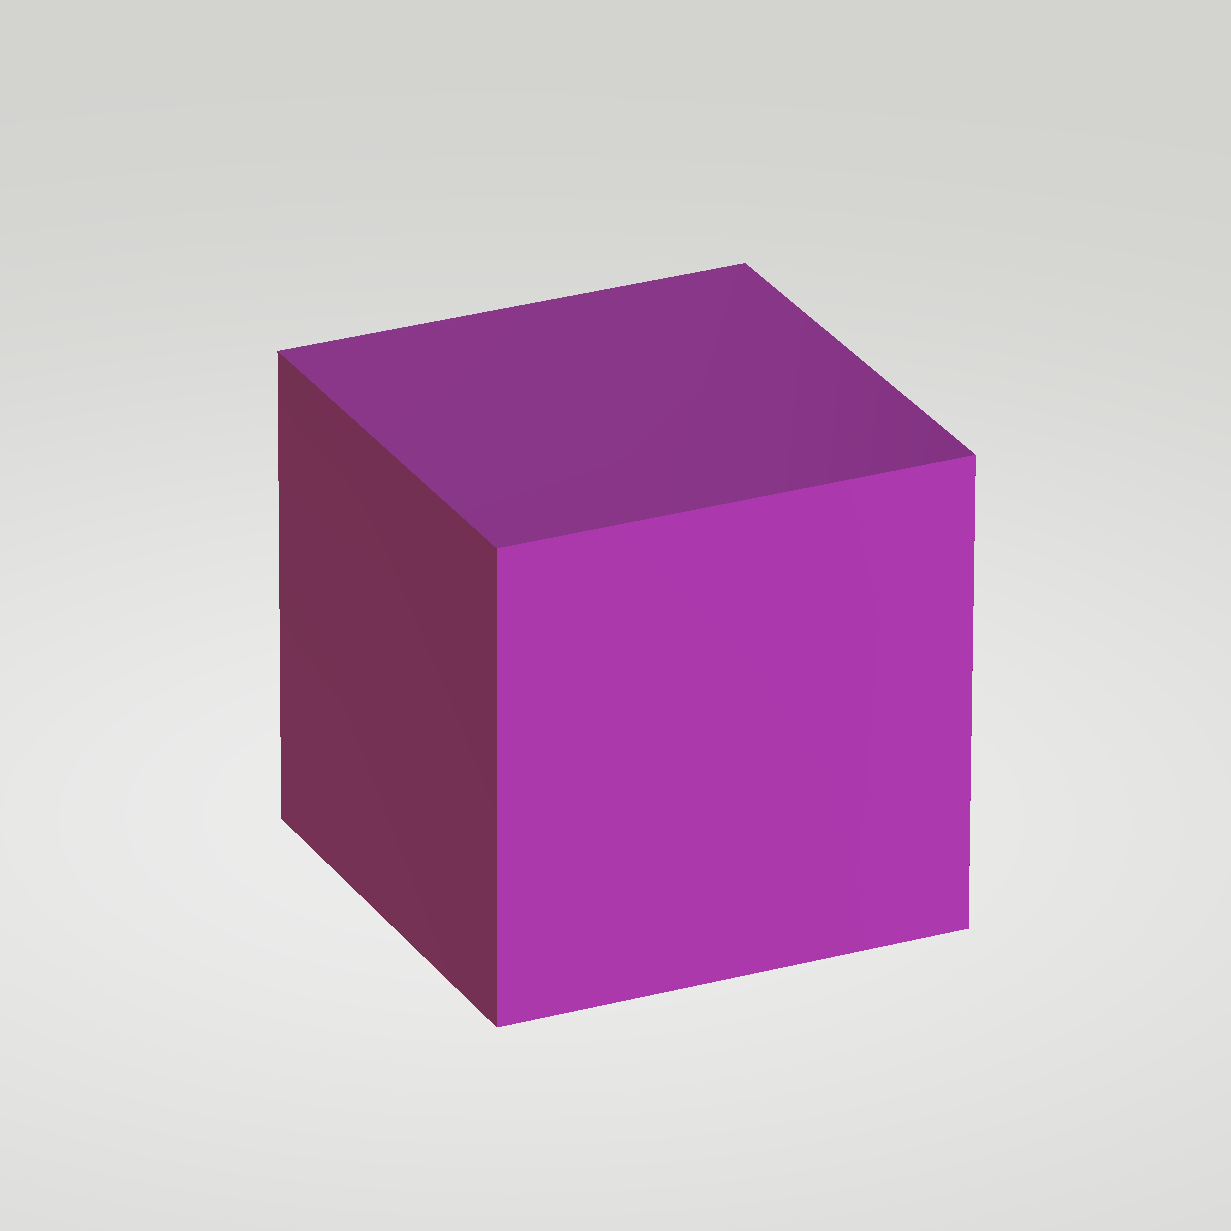
\includegraphics[width=0.24\textwidth]{resources/hexcli_step0.png}
        \hfill
        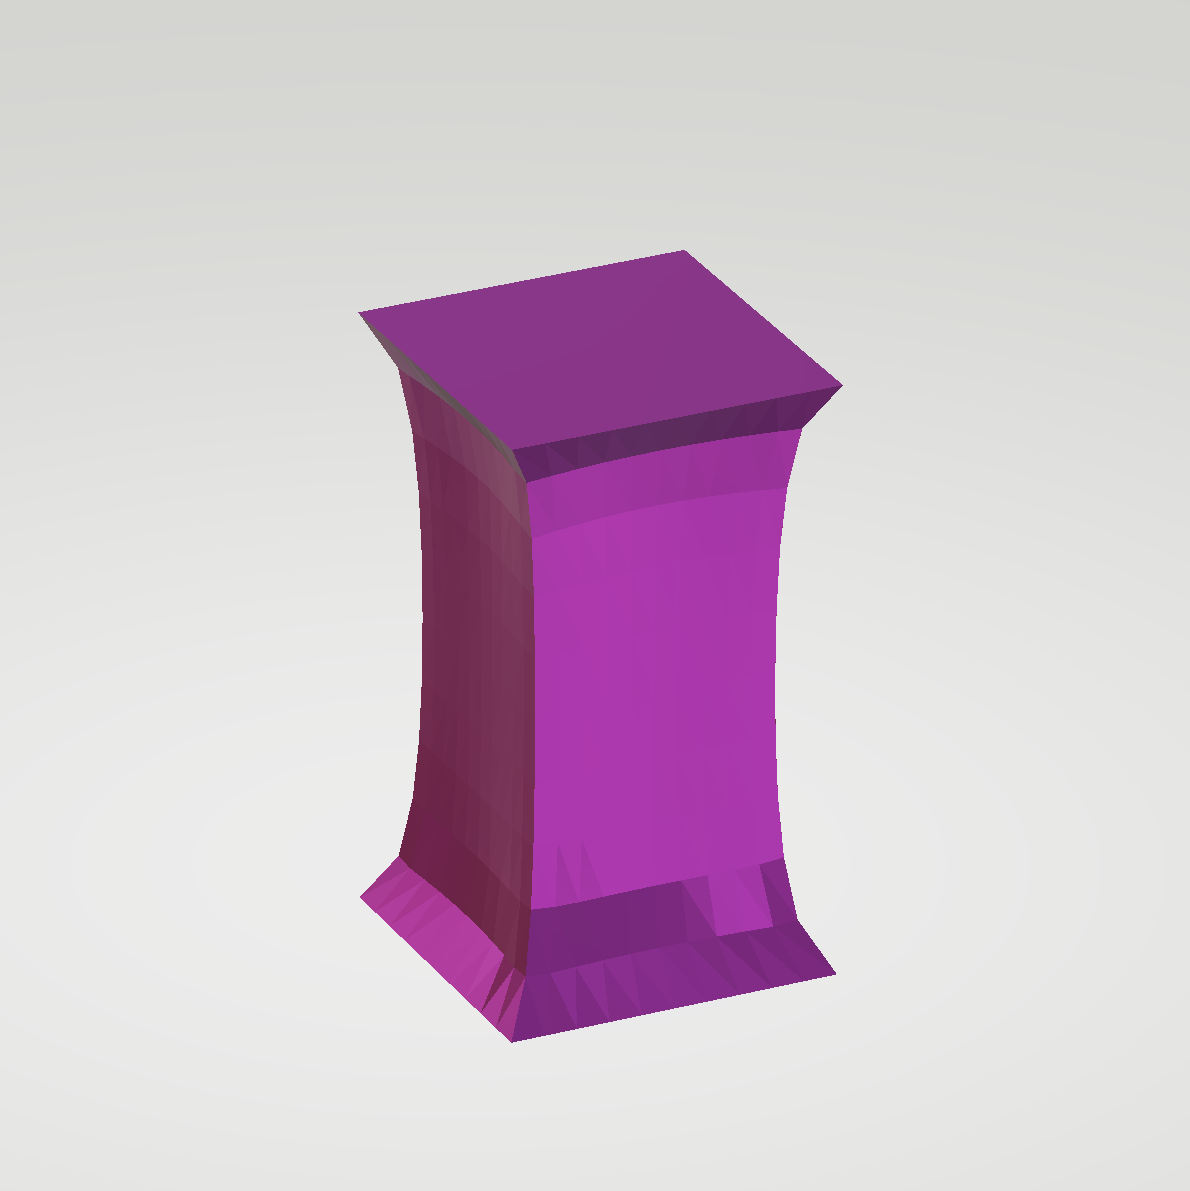
\includegraphics[width=0.24\textwidth]{resources/hexcli_step8.png}
        \hfill
        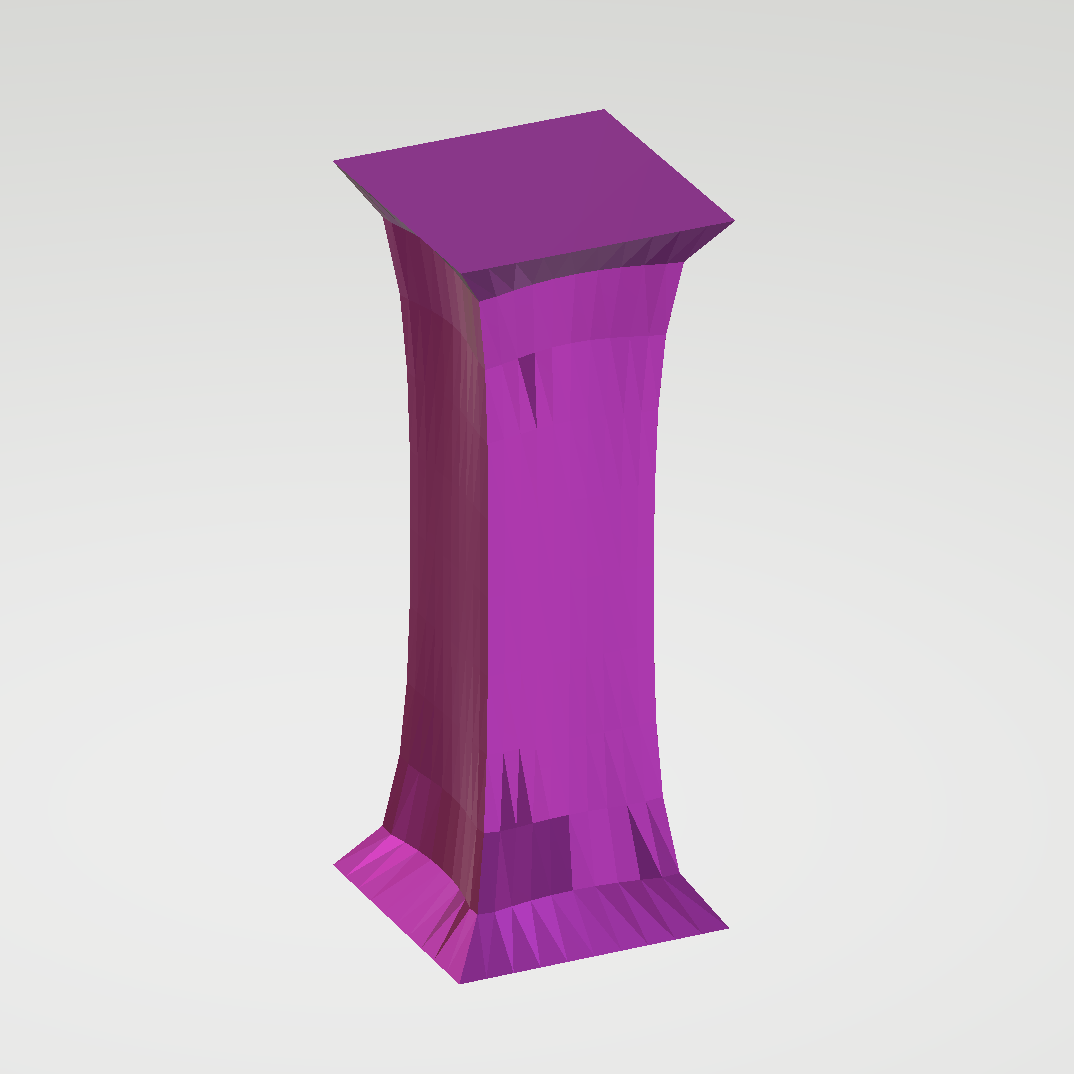
\includegraphics[width=0.24\textwidth]{resources/hexcli_step16.png}
        \hfill
        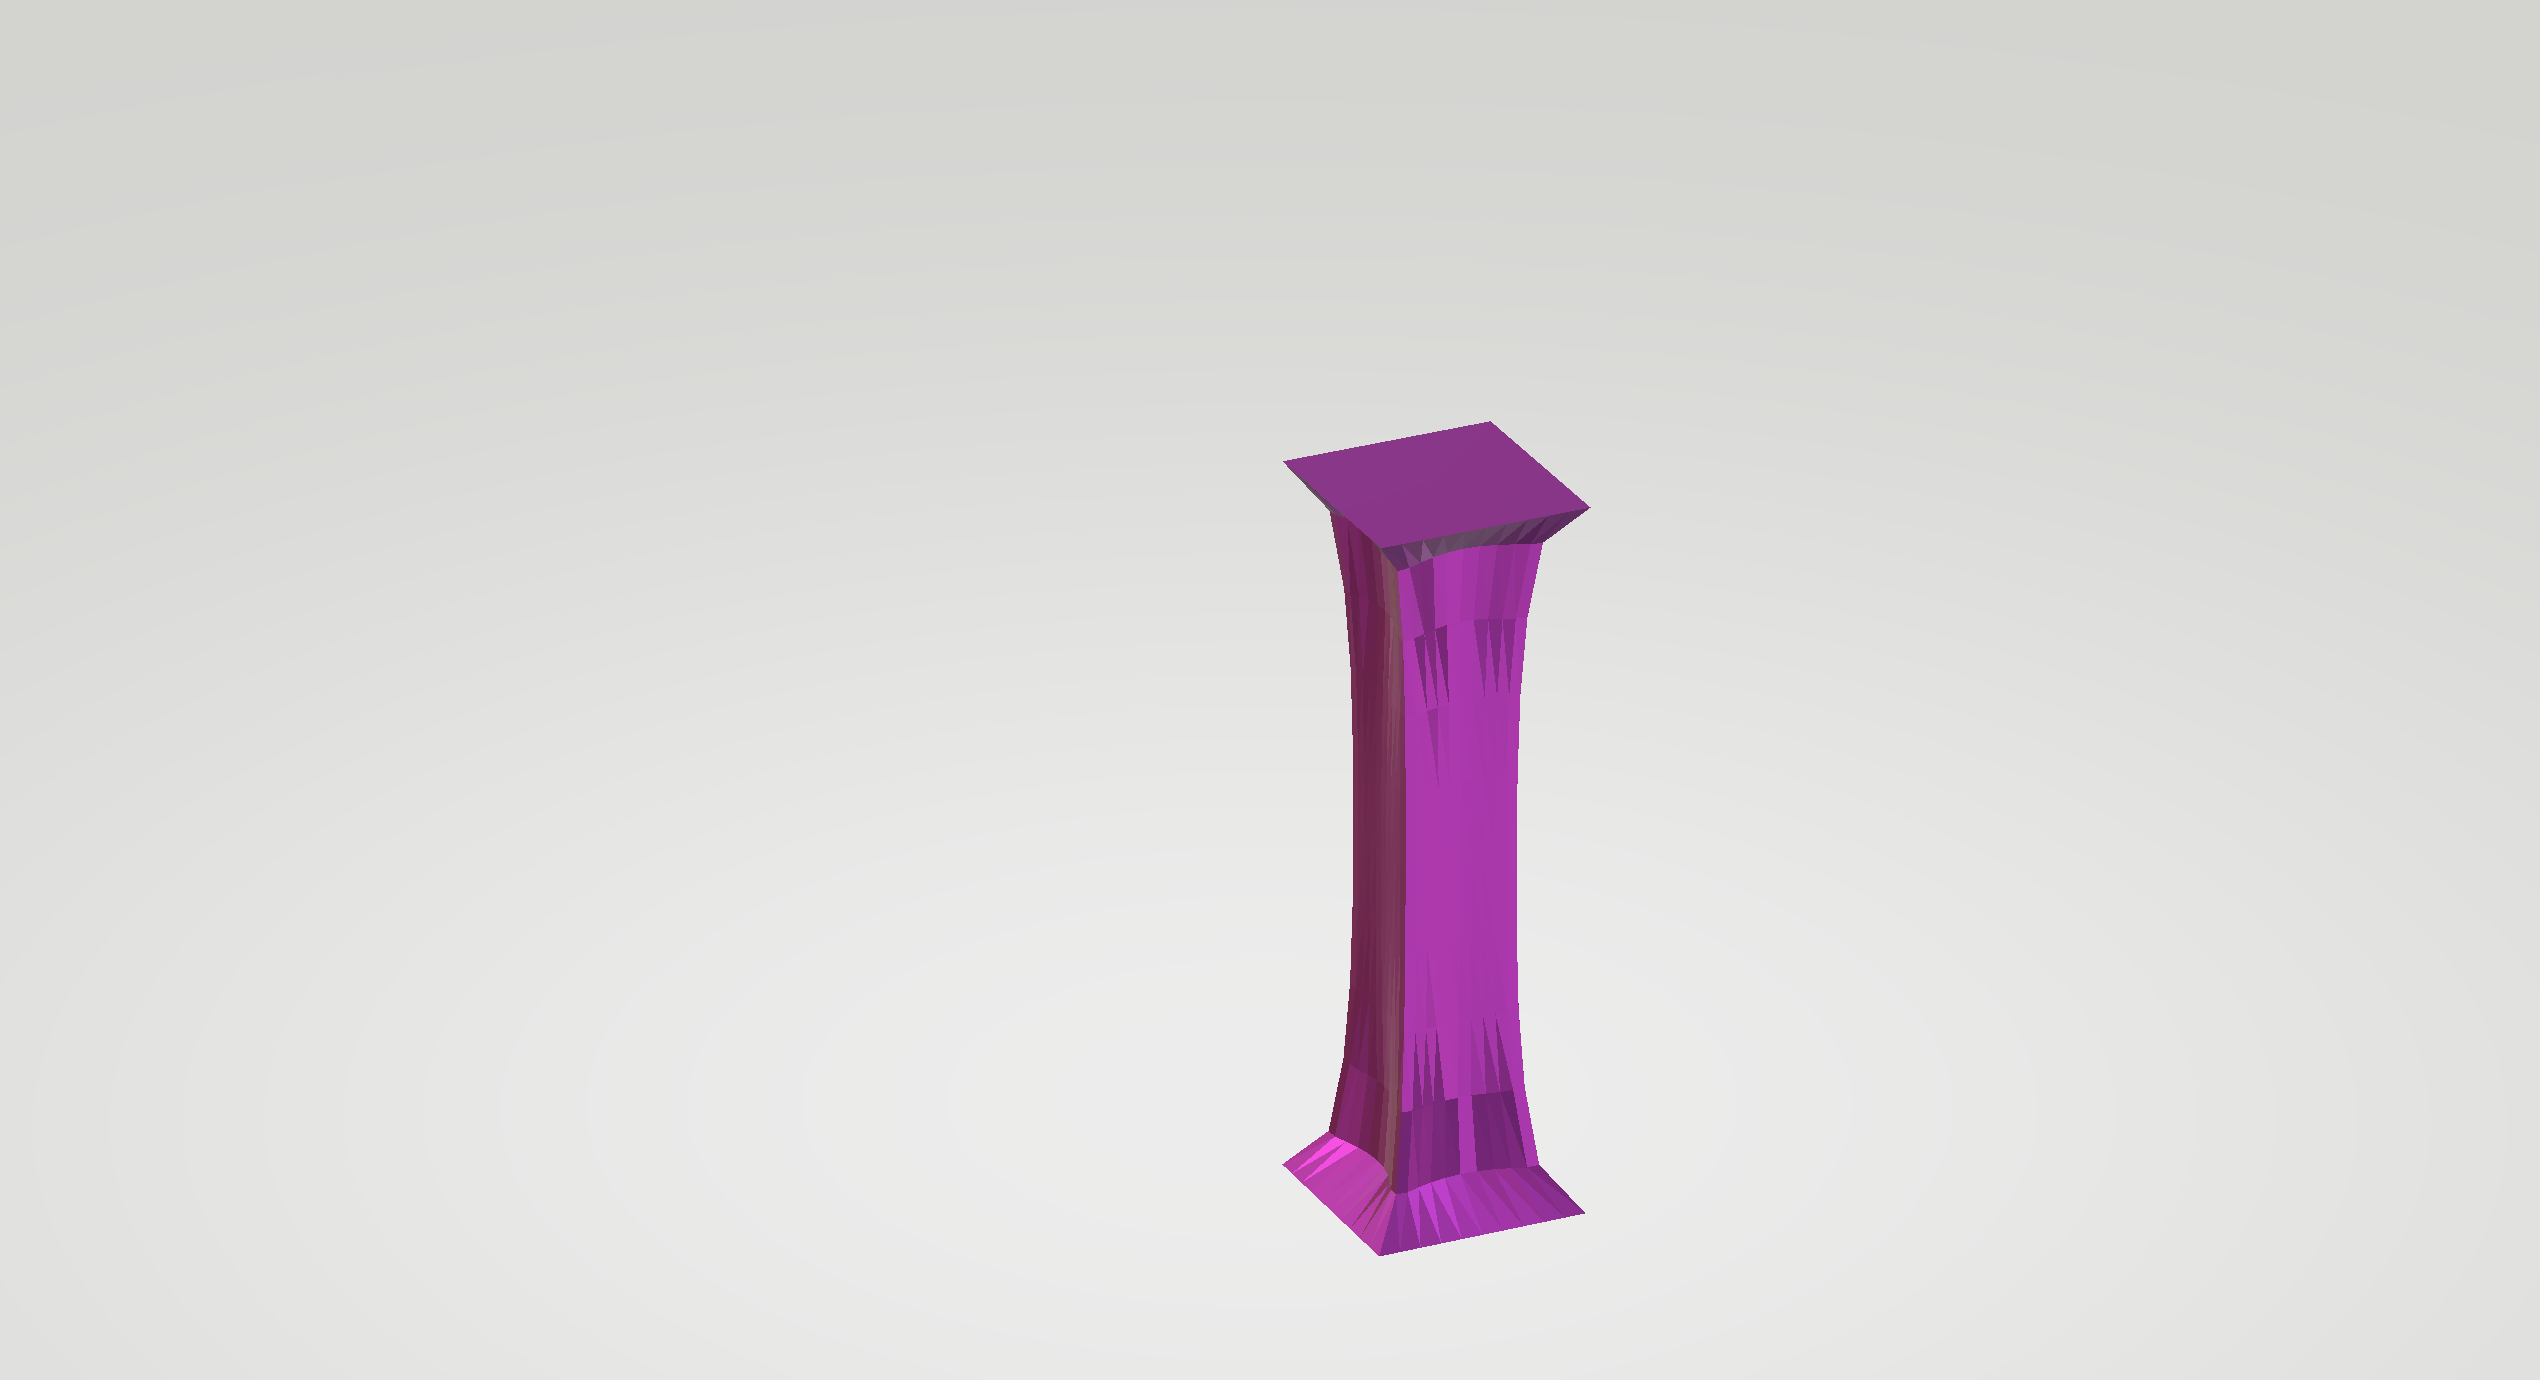
\includegraphics[width=0.24\textwidth]{resources/hexcli_step24.png}
        \caption{Stretch test on a hexahedral mesh}
    \end{subfigure}
    \vskip\baselineskip
    \begin{subfigure}[b]{\textwidth}
        \centering
        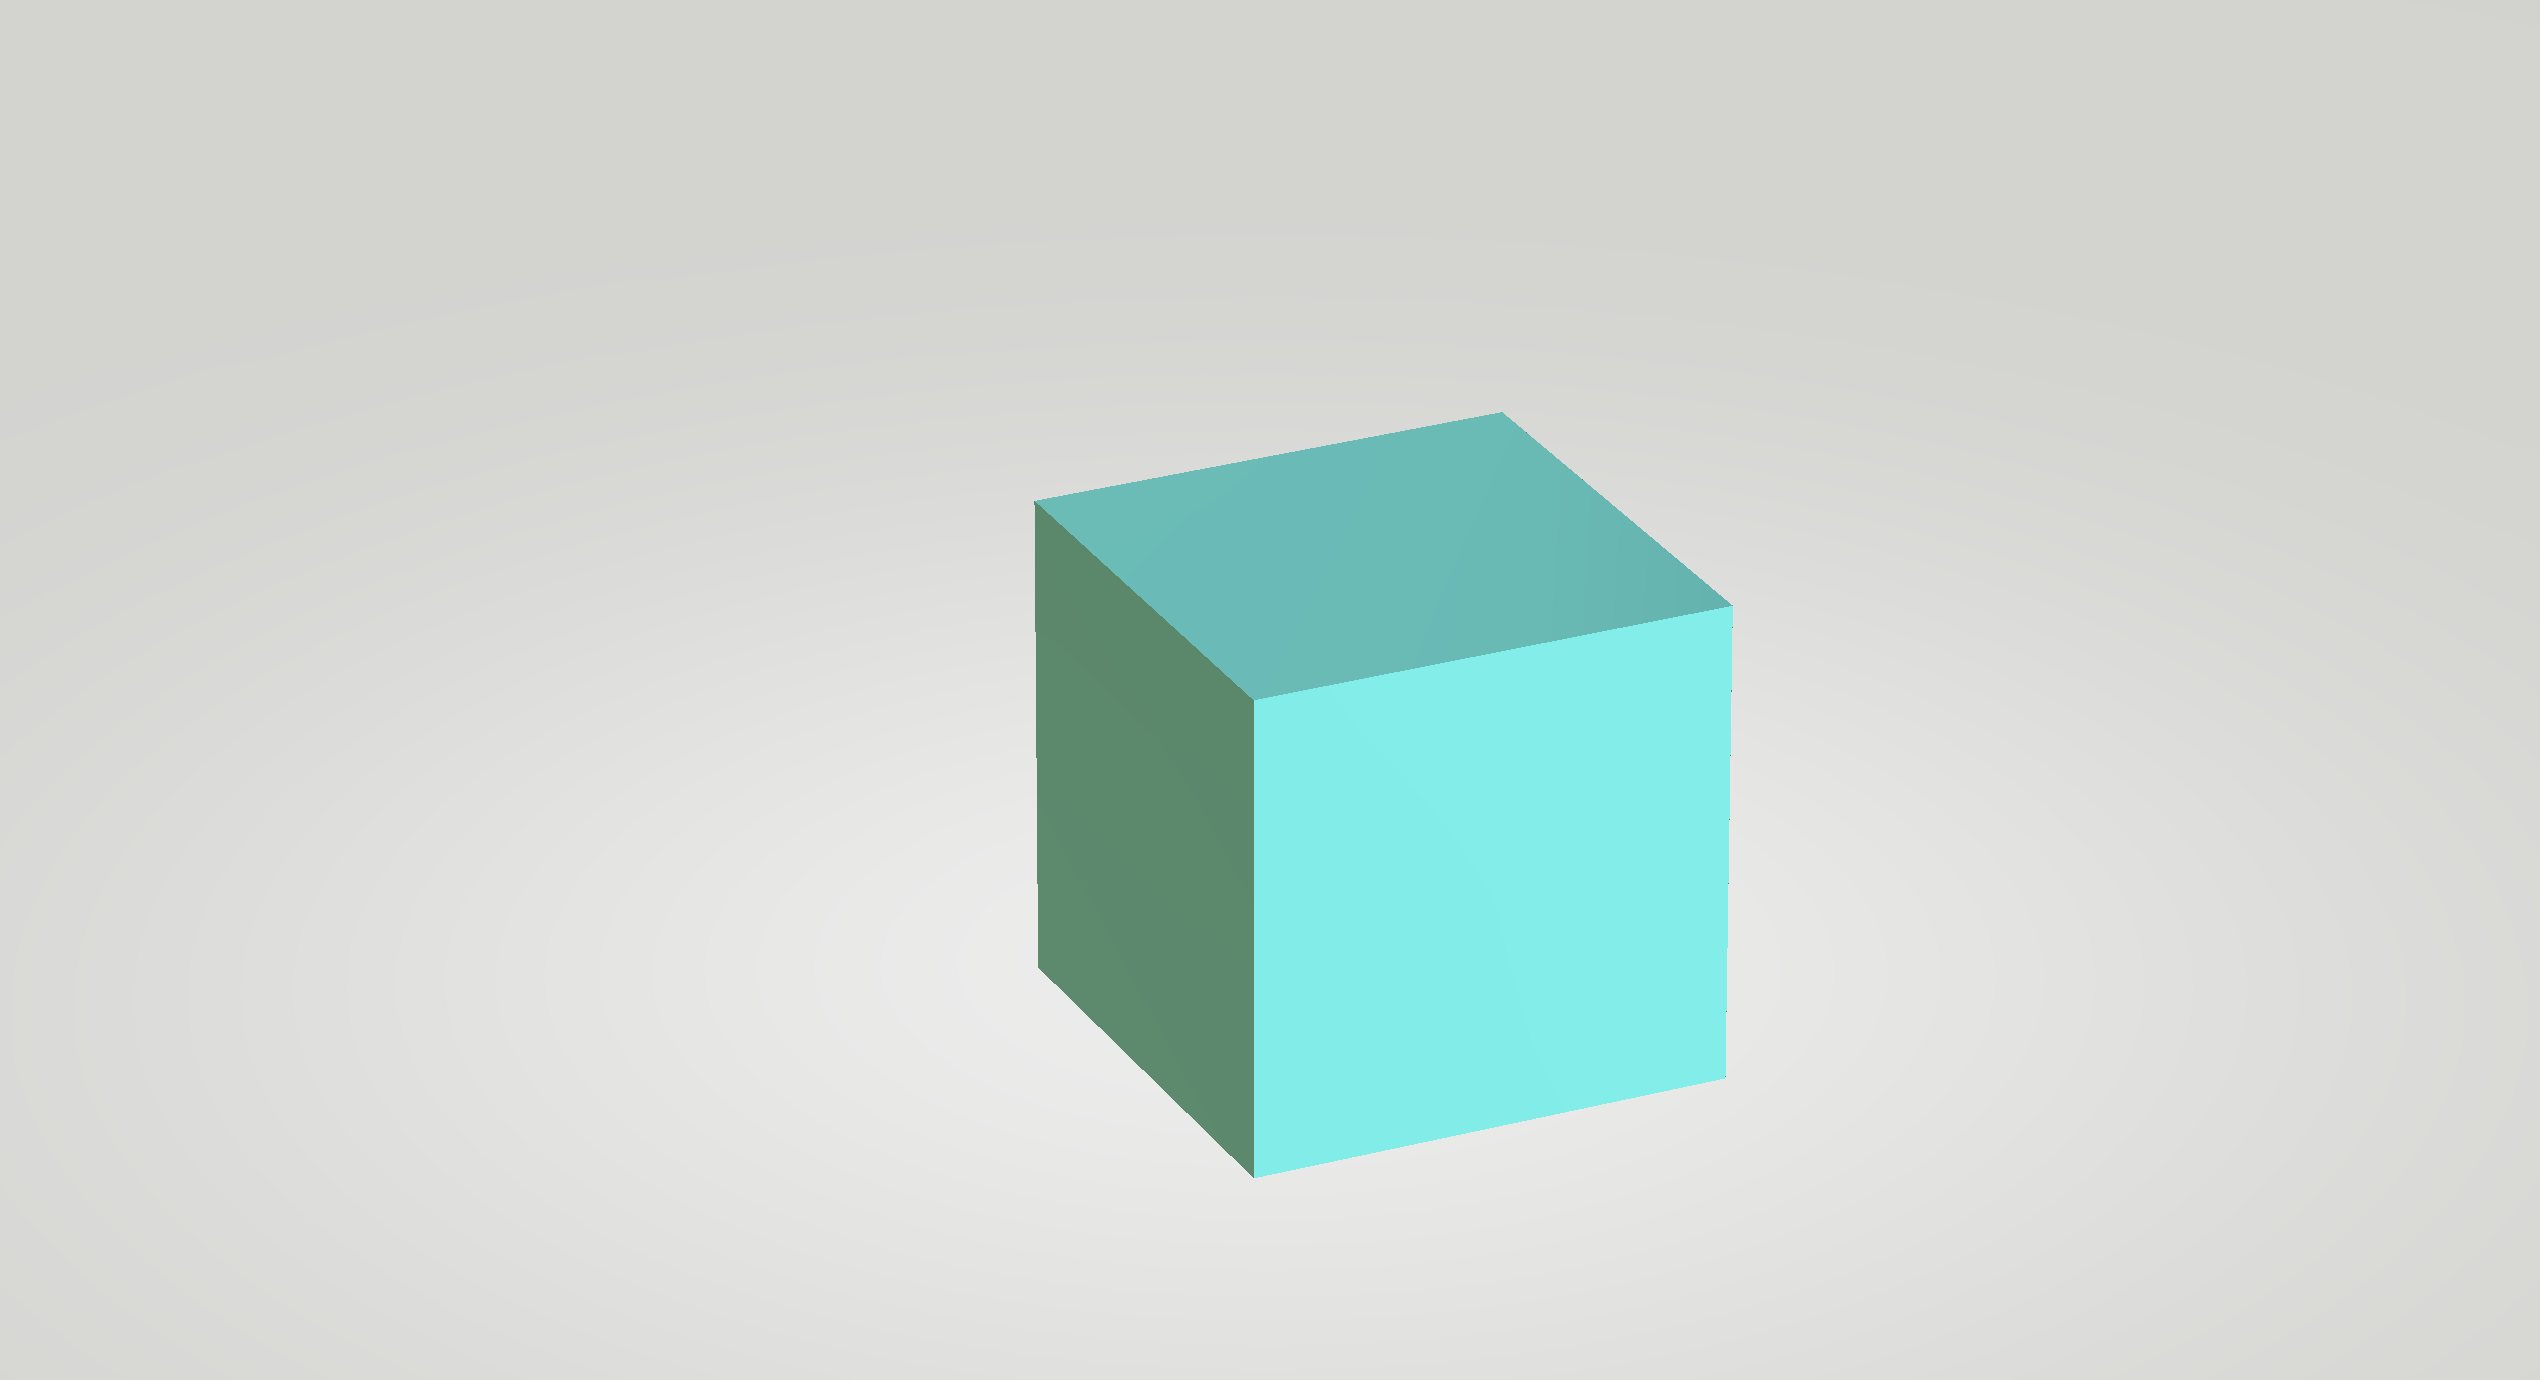
\includegraphics[width=0.24\textwidth]{resources/tetcli_step0.png}
        \hfill
        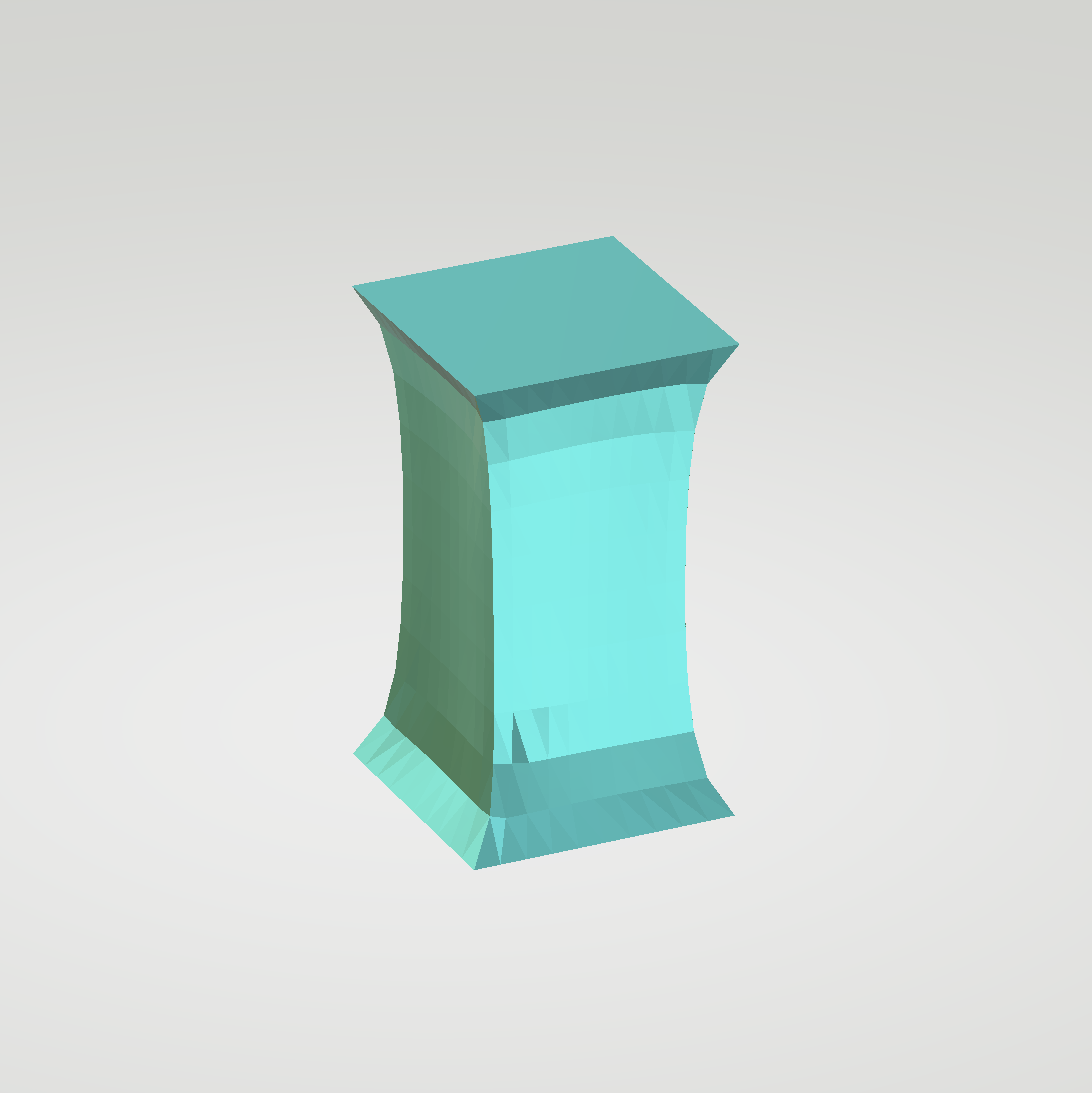
\includegraphics[width=0.24\textwidth]{resources/tetcli_step8.png}
        \hfill
        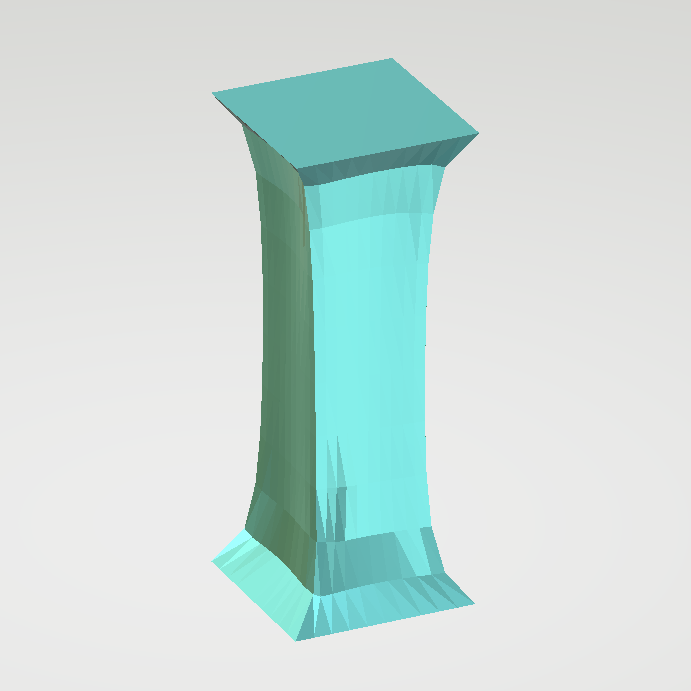
\includegraphics[width=0.24\textwidth]{resources/tetcli_step16.png}
        \hfill
        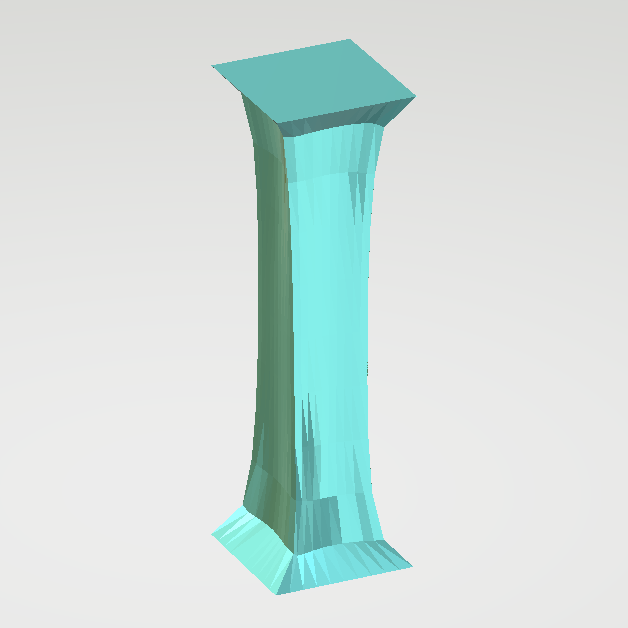
\includegraphics[width=0.24\textwidth]{resources/tetcli_step24.png}
        \caption{Stretch test on a tetrahedral mesh}
    \end{subfigure}
    \caption{Stretch test performed on a cube with (a) a hexahedral mesh and (b) a tetrahedral mesh}
    \label{fig:stretchtest}
\end{figure}


\todoredefined[inline]{
TODO: Load into OpenFlipper and screenshot results. Include more examples and what went right and what went wrong.
}



\section{Discussion}
Stuff, Taylor approx.


